% CREATED BY DAVID FRISK, 2014
\chapter{Introduction}

In 2010 Gartner estimated the global accumulated Technical Debt to be US\$ 500 billion \cite{costOfTechnicalDebt} and that it has the potential to double by the end of 2015. These numbers give an insight of the relevance of this subject that lately, as shown in \ref{fig:technical_debt_trend}, both Academia and Industry started approaching it.

Technical Debt is a metaphor borrowed from the financial world used to described short time expedients and the adoption of sub-optimal decisions which inflate software cost over time \cite{first_mention_of_TD}. As in financial debt, technical debt is tied with the concept of interest. It represents the difference in cost needed to successfully maintain the actual solution and an optimal one \cite{technicalDebtInterest}. As described in \cite{mapping_study_td, exploration_of_td, exploration_of_td2}, Techincal Debt accrues in every aspect of the Software's lifecycle and side effects of correlations between these different sub-dimension are often hard to identify and/or quantify.

Moreover, as highlighted in \ref{related_work}, the available body of knowledge still fails to identify similarities and differences between a set of these dimensions. In particular, there are no prior studies about framing the problem of Test Code Quality within the available Technical Debt frameworks despite having other studies highlighting this kinds of problem.

However, a simplicistic map of the available knowledge about Source Code Technical Debt to Test Code don't consider aspect Testware specific. I.e.\ testing comes after conventional developing activities in the Software Development pipeline and serves a different purpose. Furthermore, mainteneance activities on test code base have more triggering factors. Namely: 1) Requirements, 2) Requirements that interess the Software Source Code, 3) Refactoring of Software Source Code, and 4) Refactoring of the available test-suite. Therefore the available knowledge about indentifying and quantifying Technical Debt will result in understimate assessment of both Debt and Repayment of the the Interest.

Another aspect in which Test Code differs from Source Code consists of the different purpose of these aspects of Software. Firstly, the Test stacks span from function level tests to system ones, usually covering everything in-between. Moreover, the gaining traction of test automation require test suites to be more resilient towards Software Changes to not interrupt quality assurance processes.

For these reasons I stated the following Research Question in order to create a basic understanding of this phenomenon:
\begin{itemize}
    \item \textbf{RQ1:} What aspects of Test Code suffer the Source Code Technical Debt?
    \item \textbf{RQ2:} Is there any source of Technical Debt that is unique for Test Code?
    \item \textbf{RQ3:} For the elements identified in RQ1 and RQ2, what is the related Interest?
\end{itemize}
To answer these questions I adopted the Exploratory Case Study research methodology which will be performed in Industry settings.

\begin{figure}[h]
    \centering
    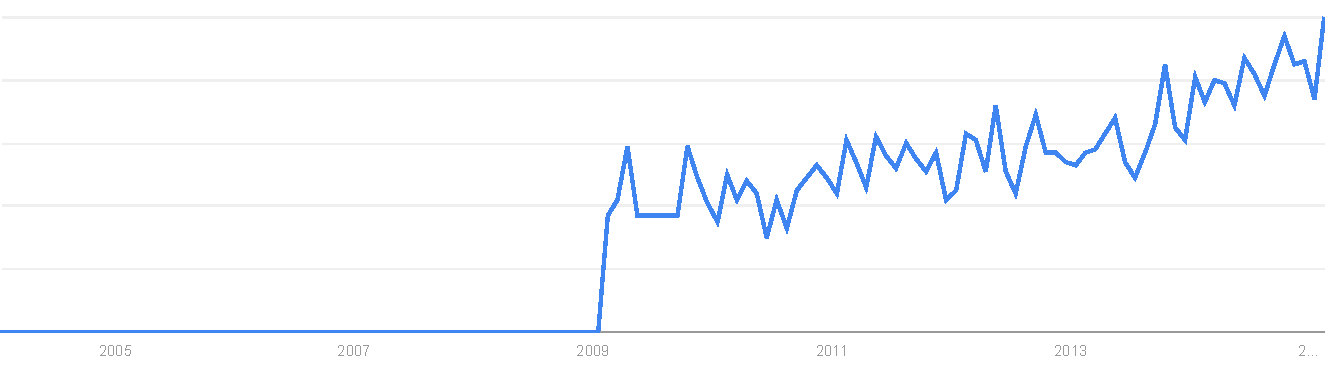
\includegraphics[width=\textwidth]{figure/technicalDebt.pdf}
    \caption{Popularity of \textit{Technical Debt} in Google over time.}
    \label{fig:technical_debt_trend}
\end{figure}

The report is articulated as follows. Section \ref{related_work} presents the relevant related work available to date on the topic. Section 3 contains an accurate description of the research methodology followed. Section 4 illustrates the data that has been gathered which is subsequently analyzed and discussed in Section 5. Section 6 contains the conclusions and possible future works on the topic. Finally, Section 7 will discuss Threats to Validity and all the steps taken to lessen them.


